\documentclass[]{article}
\pagenumbering{gobble}
\usepackage[a3paper, total={6in, 8in}]{geometry}

\usepackage{pgfplots}
\usepackage{tcolorbox}
\usepackage{circuitikz}
\usepackage{amsmath}
\usepackage{pgfplotstable}
\pgfplotsset{compat=1.18}

\usepackage{tikz}
\usetikzlibrary{automata, positioning, arrows, calc}

\tikzset{
	->,
	>=stealth,
	node distance=3cm,
	every state/.style={thick, fill=gray!10},
	initial text=$ $,
}

%opening
\title{Paper assignement 2: Alternating bit protocol}
\author{Gabriel PEREIRA DE CARVALHO}
\date{Last modification: \today}

\begin{document}
	
	\maketitle
	
	%\section{State machine for receiver}
	
	\begin{figure}[h]
		\centering
		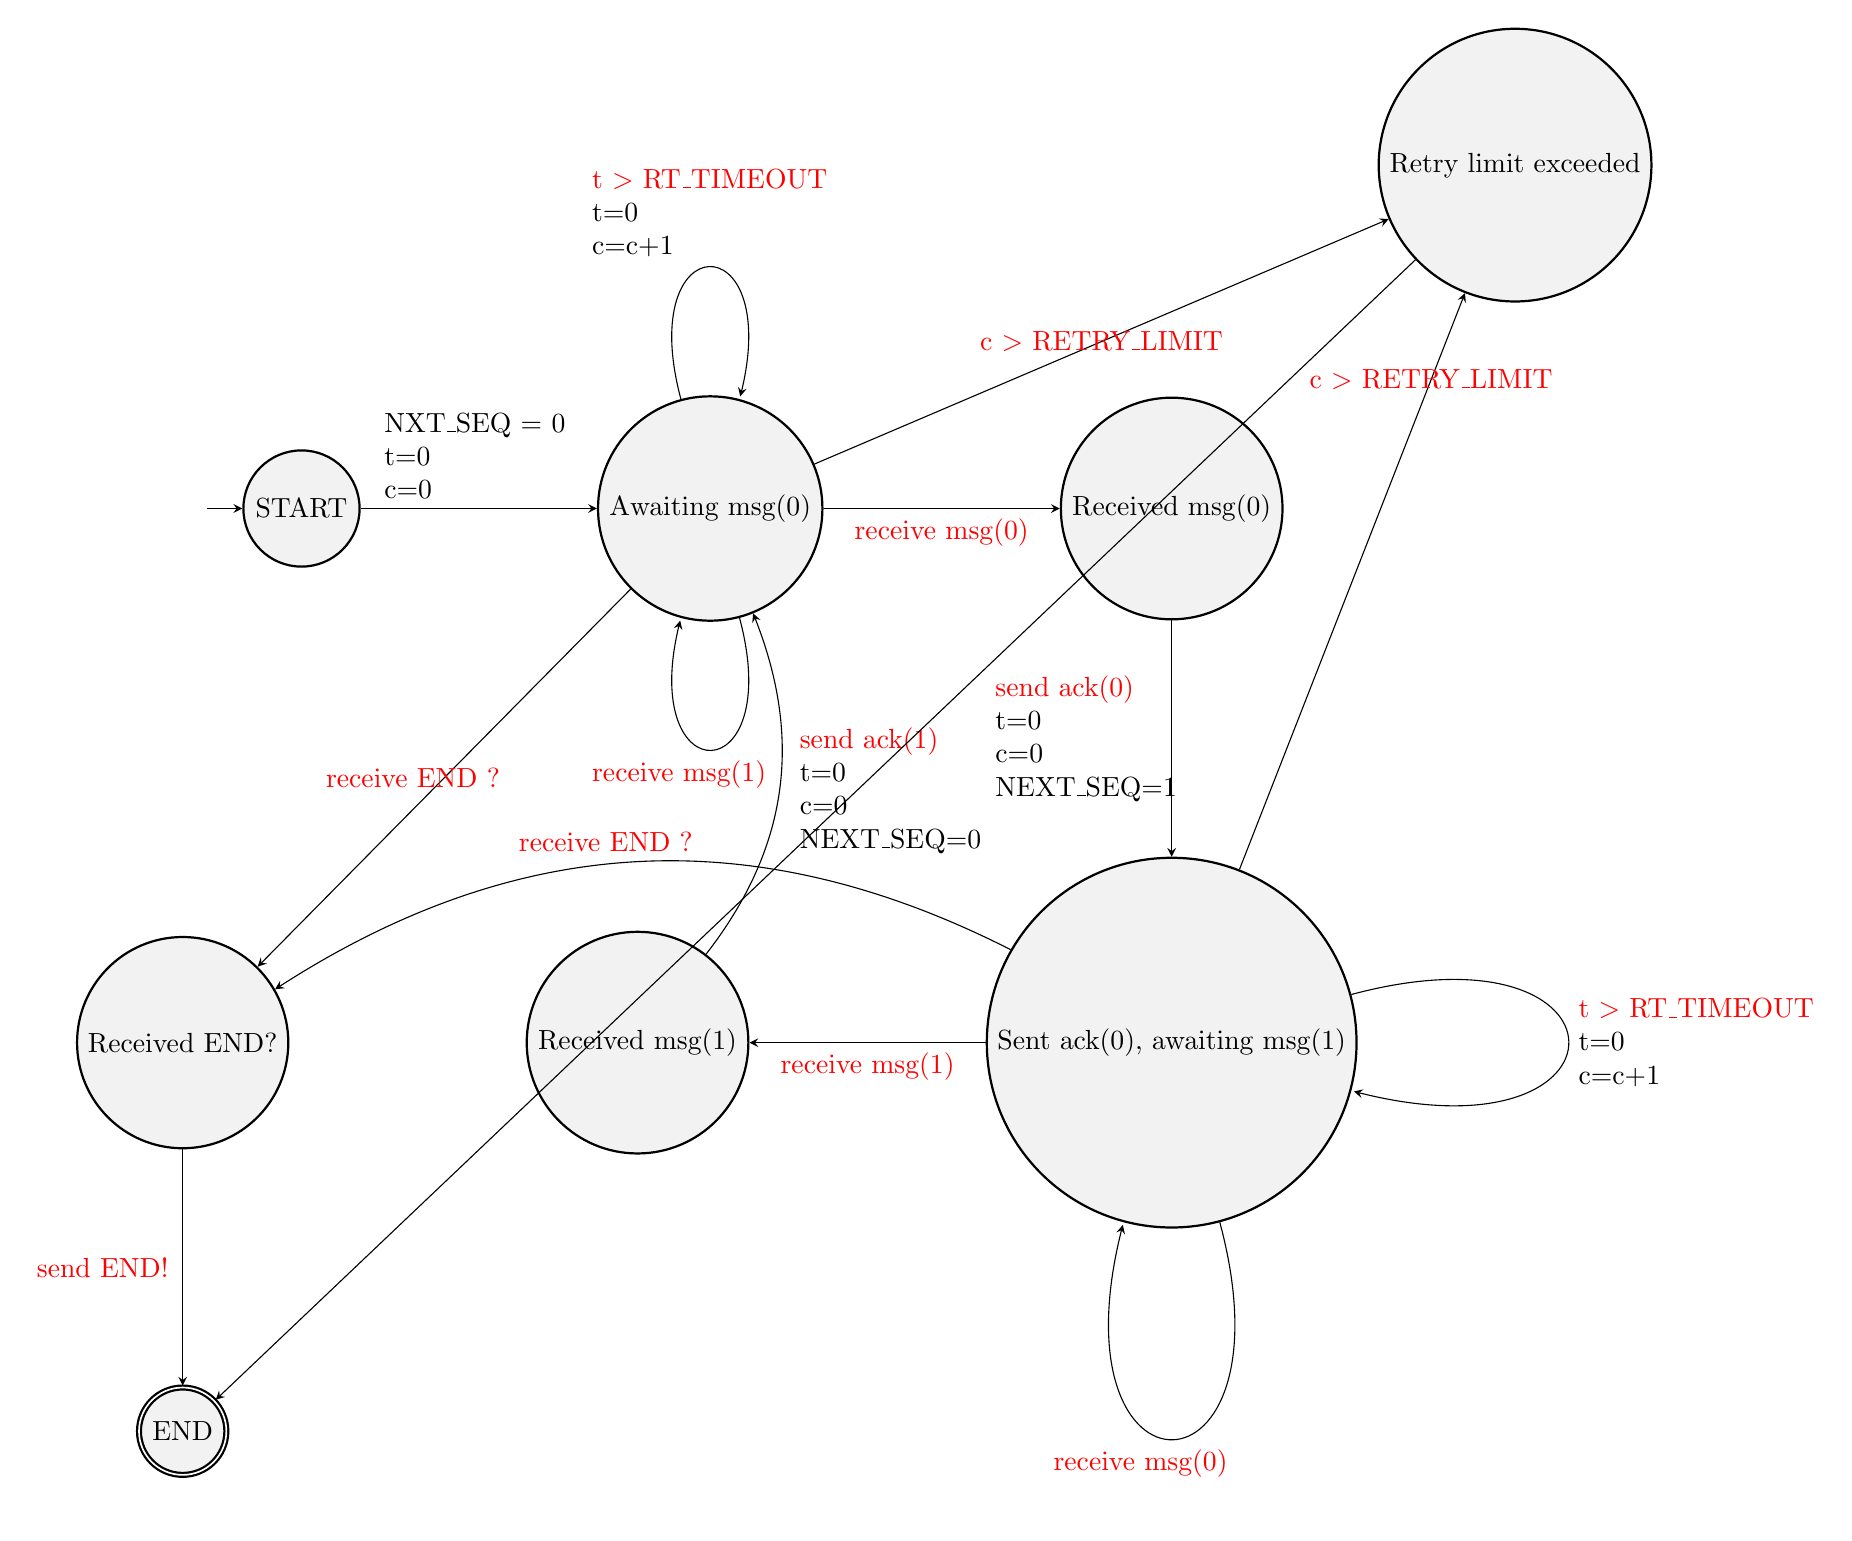
\begin{tikzpicture}
			
			\node[state, initial] (START) {START};
			\node[state, right=of START] (AWAIT0) {Awaiting msg(0)};
			\node[state, right=of AWAIT0] (REC0) {Received msg(0)};
			\node[state, above right=of REC0] (RETRYLIM) {Retry limit exceeded};
			\node[state, below=of REC0] (AWAIT1) {Sent ack(0), awaiting msg(1)};
			\node[state, left=of AWAIT1] (REC1) {Received msg(1)};
			\node[state, left=of REC1] (RECend) {Received END?};
			\node[state, accepting, below=of RECend] (END) {END};
			
			\draw (START) edge[] node[pos=0.6, above]{\parbox{3cm}{NXT\_SEQ = 0 \\ t=0 \\ c=0}} (AWAIT0);
			\draw (AWAIT0) edge[loop above] node[]{\parbox{3cm}{\textcolor{red}{t $>$ RT\_TIMEOUT} \\ t=0 \\ c=c+1}} (AWAIT0);
			\draw (AWAIT0) edge[loop below] node[]{\parbox{3cm}{\textcolor{red}{receive msg(1)}}} (AWAIT0);
			\draw (AWAIT0) edge[] node[]{\textcolor{red}{c $>$ RETRY\_LIMIT}} (RETRYLIM);
			\draw (AWAIT0) edge[] node[below]{\textcolor{red}{receive msg(0)}} (REC0);
			\draw (REC0) edge[] node[xshift = -21]{\parbox{3cm}{\textcolor{red}{send ack(0)} \\ t=0 \\ c=0 \\ NEXT\_SEQ=1}} (AWAIT1);
			\draw (AWAIT1) edge[loop right] node[]{\parbox{3cm}{\textcolor{red}{t $>$ RT\_TIMEOUT} \\ t=0 \\ c=c+1}} (AWAIT1);
			\draw (AWAIT1) edge[loop below] node[]{\parbox{3cm}{\textcolor{red}{receive msg(0)}}} (AWAIT1);
			\draw (AWAIT1) edge[] node[pos = 0.85]{\textcolor{red}{c $>$ RETRY\_LIMIT}} (RETRYLIM);
			\draw (AWAIT1) edge[] node[below]{\textcolor{red}{receive msg(1)}} (REC1);
			\draw (REC1) edge[bend right] node[xshift=50]{\parbox{3cm}{\textcolor{red}{send ack(1)} \\ t=0 \\ c=0 \\ NEXT\_SEQ=0}} (AWAIT0);
			\draw (AWAIT0) edge[] node[]{\parbox{3cm}{\textcolor{red}{receive END ?}}} (RECend);
			\draw (AWAIT1) edge[bend right] node[above]{\parbox{3cm}{\textcolor{red}{receive END ?}}} (RECend);
			\draw (RECend) edge[] node[xshift=-10]{\parbox{3cm}{\textcolor{red}{send END!}}} (END);
			
			\draw (RETRYLIM) edge[] node[]{} (END);
						
		\end{tikzpicture}
	\end{figure}
	
	\newpage
	
	%\section{Message-flow chart for Alternating Bit Protocol}
	\begin{figure}
		\centering
		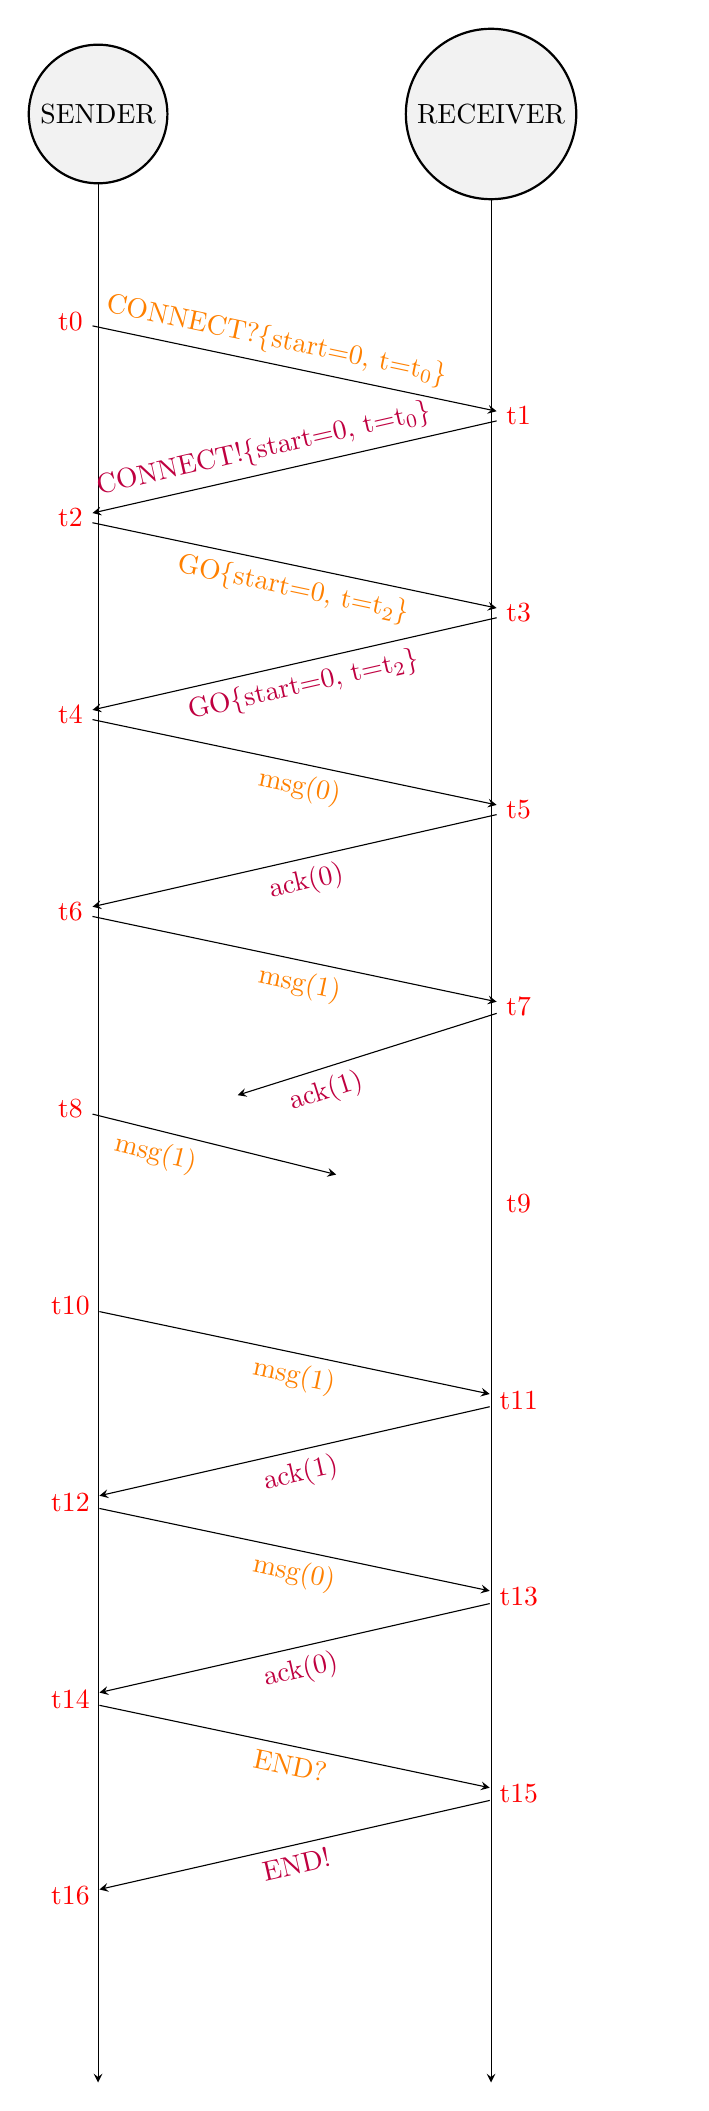
\begin{tikzpicture}
			
			\node[state] (SENDER) {SENDER};
			\node[state, right=of SENDER] (RECEIVER) {RECEIVER};
			\node[below=1.5cm of SENDER, xshift=-10] (t0) {\textcolor{red}{t0}};
			\node[below=2.5cm of RECEIVER, xshift=10] (t1) {\textcolor{red}{t1}};
			\node[below=4cm of SENDER, xshift=-10] (t2) {\textcolor{red}{t2}};
			\node[below=5cm of RECEIVER, xshift=10] (t3) {\textcolor{red}{t3}};
			\node[below=6.5cm of SENDER, xshift=-10] (t4) {\textcolor{red}{t4}};
			\node[below=7.5cm of RECEIVER, xshift=10] (t5) {\textcolor{red}{t5}};
			\node[below=9cm of SENDER, xshift=-10] (t6) {\textcolor{red}{t6}};
			\node[below=10cm of RECEIVER, xshift=10] (t7) {\textcolor{red}{t7}};
			\node[shift={(2cm, -12.5cm)}, xshift=-10] (t75) {};
			\node[below=11.5cm of SENDER, xshift=-10] (t8) {\textcolor{red}{t8}};
			\node[below=12.5cm of RECEIVER, xshift=10] (t9) {\textcolor{red}{t9}};
			\node[shift={(3.5cm, -13.5cm)}, xshift=-10] (t95) {};
			\node[below=14cm of SENDER, xshift=-10] (t10) {\textcolor{red}{t10}};
			\node[below=15cm of RECEIVER, xshift=10] (t11) {\textcolor{red}{t11}};
			\node[below=16.5cm of SENDER, xshift=-10] (t12) {\textcolor{red}{t12}};
			\node[below=17.5cm of RECEIVER, xshift=10] (t13) {\textcolor{red}{t13}};
			\node[below=19cm of SENDER, xshift=-10] (t14) {\textcolor{red}{t14}};
			\node[below=20cm of RECEIVER, xshift=10] (t15) {\textcolor{red}{t15}};
			\node[below=21.5cm of SENDER, xshift=-10] (t16) {\textcolor{red}{t16}};
			
			\draw (SENDER) -- ++(0,-25cm);
			\draw (RECEIVER) -- ++(0, -25cm);
			\draw (t0) edge[] node[sloped, above]{\parbox{5cm}{\textcolor{orange}{CONNECT?\{start=0, t=t$_0$\}}}} (t1);
			\draw (t1) edge[] node[sloped, above]{\parbox{5cm}{\textcolor{purple}{CONNECT!\{start=0, t=t$_0$\}}}} (t2);
			\draw (t2) edge[] node[sloped, below,pos=0.7]{\parbox{5cm}{\textcolor{orange}{GO\{start=0, t=t$_2$\}}}} (t3);
			\draw (t3) edge[] node[sloped, below,pos=0.3]{\parbox{5cm}{\textcolor{purple}{GO\{start=0, t=t$_2$\}}}} (t4);
			\draw (t4) edge[] node[sloped, below,pos=0.9]{\parbox{5cm}{\textcolor{orange}{msg(0)}}} (t5);
			\draw (t5) edge[] node[sloped, below,pos=0.1]{\parbox{5cm}{\textcolor{purple}{ack(0)}}} (t6);
			\draw (t6) edge[] node[sloped, below,pos=0.9]{\parbox{5cm}{\textcolor{orange}{msg(1)}}} (t7);
			\draw (t7) edge[] node[sloped, below,pos=0.1]{\parbox{5cm}{\textcolor{purple}{ack(1)}}} (t75);
			\draw (t8) edge[] node[sloped, below,pos=0.9]{\parbox{5cm}{\textcolor{orange}{msg(1)}}} (t95);
			\draw (t10) edge[] node[sloped, below,pos=0.9]{\parbox{5cm}{\textcolor{orange}{msg(1)}}} (t11);
			\draw (t11) edge[] node[sloped, below,pos=0.1]{\parbox{5cm}{\textcolor{purple}{ack(1)}}} (t12);
			\draw (t12) edge[] node[sloped, below,pos=0.9]{\parbox{5cm}{\textcolor{orange}{msg(0)}}} (t13);
			\draw (t13) edge[] node[sloped, below,pos=0.1]{\parbox{5cm}{\textcolor{purple}{ack(0)}}} (t14);
			\draw (t14) edge[] node[sloped, below,pos=0.9]{\parbox{5cm}{\textcolor{orange}{END?}}} (t15);
			\draw (t15) edge[] node[sloped, below,pos=0.1]{\parbox{5cm}{\textcolor{purple}{END!}}} (t16);
			
			
		\end{tikzpicture}
	\end{figure}
	

\end{document}